\section{Introduction}
\label{sec:intro}

\lipsum[2]

\subsection{Preliminaries}
\label{sec:pre}

\lipsum[3]

\subsection{Previous Results}
\label{sec:prev-results}

Null graphs are discussed in \cite{HararyR74}
The concept of ``internally stable set'' was used in \cite{Berge57, Berge58}.

\begin{theorem}
	\label{thrm:1}
	\lipsum[4]
\end{theorem}
\begin{proof}
	content...
\end{proof}

\begin{corollary}
\label{cor:1}

\lipsum[5]
\end{corollary}

Unordered List (taken from Overleaf)
\begin{itemize}
	\item The individual entries are indicated with a black dot, a so-called bullet.
	\item The text in the entries may be of any length.
\end{itemize}

Ordered List (taken from Overleaf)
\begin{enumerate}
	\item The labels consists of sequential numbers.
	\item The numbers starts at 1 with every call to the enumerate environment.
\end{enumerate}

\begin{table}[ht]
	\centering
	\begin{tabular}{|c|c|}
		\hline
		\textbf{Odd} & \textbf{Even} \\
		\hline\hline
		One & Two \\
		\hline
		Three & Four \\
		\hline
	\end{tabular}
	\caption{This is a table}
	\label{tbl:1}
\end{table}

Table~\ref*{tbl:1} is an example of a table.


\section{Methodology}
\label{sec:methods}

\section{Results}
\label{sec:results}

\section{Discussion}
\label{sec:discuss}

\section{More Examples}
\label{sec:examples}

Now we include a figure.
(See Figure~\ref{fig:example}.)
\begin{figure}[ht]
	\centering
	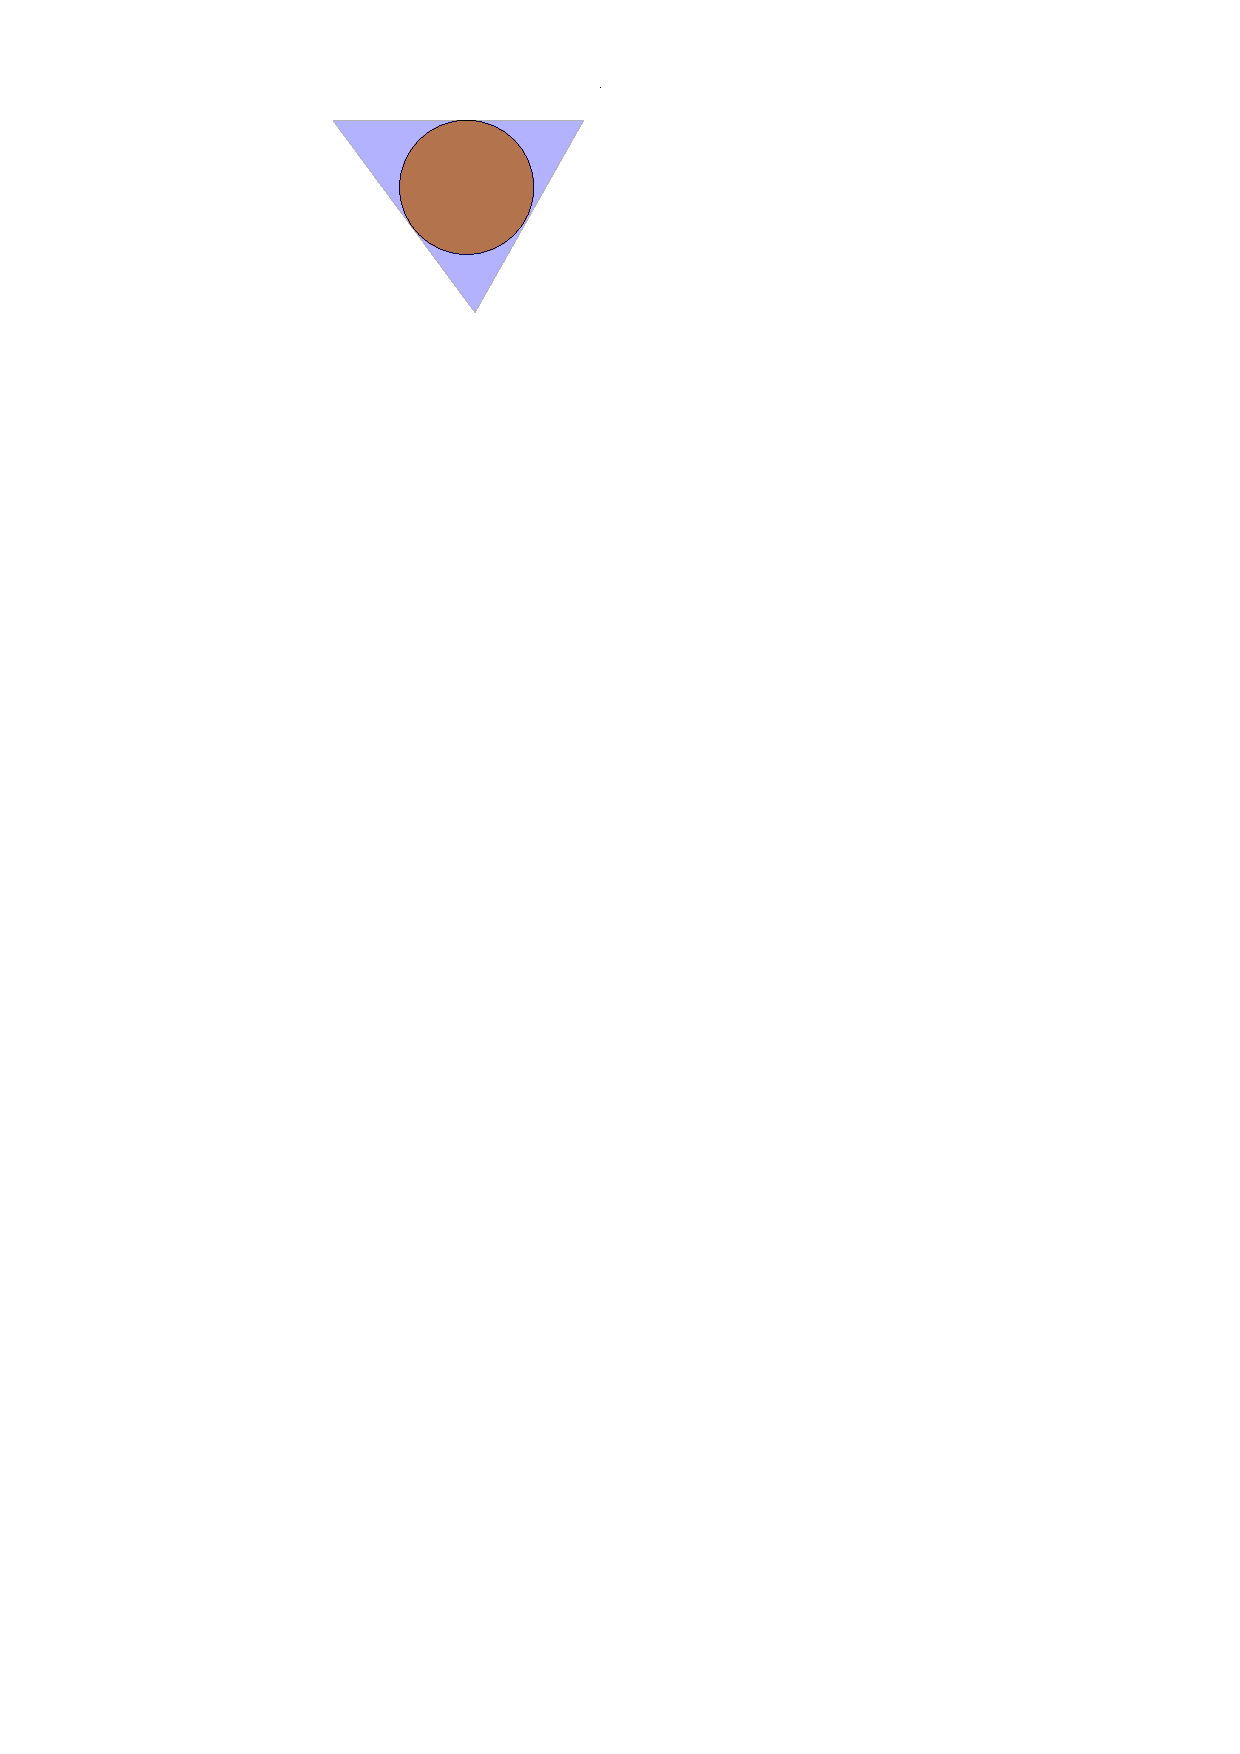
\includegraphics[width=0.3\textwidth]{example}
	\caption{An example of a figure}
	\label{fig:example}
\end{figure}

\paragraph{Acknowledgements} \lipsum[6]

%	\newpage
\bibliography{refs}

\appendix

\section{Omitted Proof in Section~\ref{sec:examples}}
\label{app:1}

\lipsum[7]